\RequirePackage{fix-cm}
\documentclass[twocolumn]{svjour3}

\smartqed

\usepackage{graphicx}

\tolerance=1
\emergencystretch=\maxdimen
\hyphenpenalty=10000
\hbadness=10000

\def\makeheadbox{\relax}

\usepackage[numbers]{natbib}
\usepackage{algorithm}
\usepackage{algpseudocode}

\renewcommand{\algorithmicrequire}{\textbf{Input:}}
\renewcommand{\algorithmicensure}{\textbf{Output:}}

\usepackage{amsmath,amssymb}
\usepackage{tabularx}
\usepackage{booktabs}
\usepackage{url}
\usepackage{tikz}
\usetikzlibrary{arrows.meta, positioning, shapes.geometric}
\usepackage[dvipsnames,table]{xcolor}
\usepackage{microtype}
\usepackage[most]{tcolorbox}

\newtcolorbox{keyresult}{
  enhanced,
  breakable,
  colback=blue!3!white,
  boxrule=0pt,
  frame hidden,
  borderline west={3pt}{0pt}{blue!45!black!65},
  left=8pt, right=5pt, top=4pt, bottom=4pt,
  before skip=3pt,
  after skip=3pt,
  sharp corners,
}

\usepackage{latexsym}
\usepackage{enumitem}
\usepackage{mathptmx}
\usepackage{pgfplots}
\pgfplotsset{compat=1.12}
\usepackage{float}
\usepackage{stfloats}



\begin{document}

\title{Empirical Characterization of Kubernetes HPA Limitations
for Stateful WebSocket Workloads}

\titlerunning{HPA Behavior Under Stateful WebSocket Workloads}

\author{
Abhash Behera \and
Aditya Hota \and
Suprit Kumar Naik \and
Ritesh Kumar Singh
}

\authorrunning{ }

\date{Received: -; Accepted: -}

\institute{
\textbf{Abhash Behera} \at
Department of Computer Science and Engineering, \\
C V Raman Global University, Bhubaneswar 752054, India \\
\email{abhasbehera320@gmail.com}
\and
\textbf{Aditya Hota} \at
Department of Computer Science and Engineering, \\
C V Raman Global University, Bhubaneswar 752054, India \\
\email{adityahota99@gmail.com}
\and
\textbf{Suprit Kumar Naik} \at
Department of Computer Science and Engineering, \\
C V Raman Global University, Bhubaneswar 752054, India \\
\email{supritkumarnaik17@gmail.com}
\and
\textbf{Ritesh Kumar Singh} \at
Department of Computer Science and Engineering, \\
C V Raman Global University, Bhubaneswar 752054, India \\
\email{rihankumar2004@gmail.com}
}

\maketitle

\begin{abstract}
The Kubernetes Horizontal Pod Autoscaler (HPA) implements a proportional control law
over CPU utilization as its primary scaling signal. An architecture that performs
reliably for stateless, request-driven workloads but is poorly matched to
stateful, persistent-connection protocols such as WebSocket. In WebSocket deployments,
the primary unit of computational commitment is an active network connection whose
session state persists independently of CPU activity; the termination of any pod
severs the connections it hosts. This paper presents
a systematic empirical characterization of HPA failure under WebSocket workloads
through a progressive chain of four controlled experiments. Experiment~A establishes
a correct-behavior baseline under the idealized condition of CPU-to-connection
proportionality. Experiment~B1 demonstrates that HPA over-provisions by 87.5\% under
cyclic load, exhausting \texttt{maxReplicas} within 99~seconds and requiring
650~seconds to recover. Experiment~B2-Instrumented uses Prometheus instrumentation
to measure reconnection storm rates causally linked to HPA scale-down decisions,
with a peak observed rate of 1,400~connections/second and a 51.9\% connection count
overshoot (1,215 vs.\ 800 target). Experiment~B3 demonstrates permanent, irrecoverable
staircase connection destruction under non-reconnecting clients, with the active session
population monotonically reduced from 800 to a mean of 649 ($\pm$8.8) across five
replications, representing 18.8\% mean connection loss with zero recovery. Our experiments
suggest that these failure modes are \textit{architectural} rather than configurational:
they arise from the limitations of CPU as a scaling signal for persistent-connection
workloads and are unlikely to be remediated by HPA parameter tuning alone. The findings
motivate the design of connection-aware autoscaling policies, as pursued in the companion
paper.

\keywords{Kubernetes \and
Horizontal Pod Autoscaler \and
WebSocket \and
Stateful Workloads \and
Autoscaling \and
Reconnection Storm \and
Cloud Computing \and
Performance Evaluations}
\end{abstract}



%% ============================================================
\section{Introduction}
\label{sec:intro}
%% ============================================================

Kubernetes has established itself as the de facto standard platform for container
orchestration, providing declarative workload management, automated scheduling, and
elastic scaling for cloud-native applications~\cite{burns2016borg,verma2015large}.
Central to its elasticity model is the \textbf{Horizontal Pod Autoscaler (HPA)}, which
evaluates observed resource metrics at a fixed synchronization interval and adjusts
replica counts through a proportional control law~\cite{k8s_hpa_docs,nguyen2020hpa}.
For stateless, request-driven workloads such as HTTP APIs, where instantaneous CPU
consumption is a reliable proxy for current demand, this approach converges stably and
performs predictably~\cite{casalicchio2019auto,lorido2014auto}.

A fundamental shift in cloud-native workload characteristics, however, increasingly
invalidates this assumption. Real-time communication systems, IoT telemetry pipelines,
collaborative editing platforms, financial data streams, and multiplayer gaming backends
rely on the WebSocket protocol~\cite{websocket_rfc} - a full-duplex, persistent-connection
transport layer in which each client maintains a long-lived TCP session with the server.
In such workloads, the primary unit of computational commitment is not a CPU cycle or a
transient HTTP transaction, but an \textit{active network connection} whose session state
may persist for minutes to hours. The termination of any pod severs the connections
it hosts, triggering a forced client reconnection cascade - a phenomenon we term a
\textbf{reconnection storm}.

This creates a significant mismatch: \textbf{CPU utilization does not encode connection
state fidelity by default}. A server sustaining 800 idle but active WebSocket sessions may
exhibit near-zero CPU utilization, yet the destruction of a single pod hosting those sessions
is disruptive to the affected clients. HPA does not distinguish an
\textit{idle-but-connected} server from a \textit{genuinely unloaded} one, and will
therefore terminate pods that are essential to live client sessions.

Prior investigations of WebSocket autoscaling, such as Dickel et al.~\cite{dickel2019evaluation},
have acknowledged the additional complexity of stateful protocols compared to stateless HTTP
workloads. However, that work neither quantifies the failure modes of CPU-based HPA with
empirical precision, nor provides a measured reconnection storm rate. This paper addresses
the characterization gap through the following contributions:

\begin{enumerate}[leftmargin=*]
\item \textbf{Progressive four-experiment evidence chain.} Experiments~A, B1,
  B2-Instrumented, and B3 form a controlled sequence that isolates and quantifies
  each HPA failure mode, progressing from over-provisioning, to reconnection storm
  measurement, to permanent connection destruction.

\item \textbf{Empirical measurement of reconnection storm magnitude.} We observe
  a peak reconnection storm rate of 1,400~connections/second as a direct causal consequence
  of an HPA scale-down decision, using Prometheus instrumentation to provide a precise,
  reproducible measurement.

\item \textbf{Causal evidence of architectural limitation.} Experiment~B3 demonstrates the
  causal chain: CPU drops to near-zero (connections become idle) $\rightarrow$ HPA scales
  down $\rightarrow$ active sessions are permanently destroyed. This is a direct consequence
  of the CPU signal's inability to encode connection state.

\item \textbf{Establishment of the stabilization window semantic mismatch.} We show that
  HPA's built-in stabilization window, which buffers metric-derived replica recommendations,
  is insufficient to protect idle connections: with persistent near-zero CPU, every window
  entry recommends \texttt{minReplicas}, and the stabilized output converges to
  \texttt{minReplicas} regardless of window duration.

\item \textbf{Quantified failure metrics as comparison baselines.} All failure modes are
  quantified at connection-second granularity (87.5\% over-provisioning, 1,400~conn/s peak
  storm, 18.8\% mean staircase connection loss), providing reproducible baselines for
  future autoscaling research in this domain.
\end{enumerate}

The remainder of this paper is structured as follows. Section~\ref{sec:related} surveys
related work. Section~\ref{sec:background} provides a concise overview of the HPA control
architecture. Section~\ref{sec:problem} presents the four-experiment evidence chain.
Section~\ref{sec:discussion} analyzes the root causes and implications.
Section~\ref{sec:limitations} discusses limitations. Section~\ref{sec:conclusion} concludes
and motivates future work.



%% ============================================================
\section{Related Work}
\label{sec:related}
%% ============================================================

\subsection{Kubernetes HPA Architecture and Behavior}

Nguyen et al.~\cite{nguyen2020hpa} provide a comprehensive architectural analysis of the
Kubernetes HPA feedback loop, characterizing the behavior of both Kubernetes Resource Metrics
(KRM) and Prometheus Custom Metrics (PCM) pipelines across diverse scaling configurations.
Their work demonstrates that metric pipeline choice - particularly the Prometheus scrape
interval - materially affects HPA responsiveness and scaling accuracy. The present paper
extends their analysis to the \textit{stateful workload} domain, a scenario their framework
did not evaluate.

Casalicchio and Perciballi~\cite{casalicchio2019auto} demonstrated that the choice between
relative and absolute metrics directly determines scaling stability, but confined their
evaluation to CPU and memory signals for HTTP workloads. Lorido-Botr{\'a}n et
al.~\cite{lorido2014auto} provide a broader survey of auto-scaling techniques in cloud
environments, establishing the theoretical framing of proportional controllers that this
paper applies to persistent-connection workloads.

\subsection{Custom and Application-Level Metrics for HPA}

Kubernetes supports application-defined scaling signals through the Prometheus
Adapter~\cite{prometheus_adapter}, enabling HPA to react to metrics beyond CPU. Qu et
al.~\cite{qu2018auto} surveyed HTTP-rate-based autoscaling; Rossi et al.~\cite{rossi2020horizontal}
studied hybrid CPU-and-traffic strategies. However, all these formulations presuppose that
the scaling metric is \textit{stateless across pod boundaries} - an assumption violated
by connection-holding protocols where session state is affined to a specific pod instance.
Furthermore, even when HPA is configured with a correct connection-count metric via the
Prometheus Adapter, HPA's stabilization semantics remain CPU-oriented: the window stabilizes
metric-derived replica recommendations rather than connection-derived desired counts. This
distinction is analyzed in Section~\ref{sec:discussion} and evaluated experimentally in the
companion paper.

\subsection{Stateful Workloads and Protocol-Aware Autoscaling}

Dickel et al.~\cite{dickel2019evaluation} identified stateful autoscaling as an open research
challenge specific to IoT gateway deployments using WebSocket and MQTT. While their work
motivates the need for protocol-aware scaling and proposes monitoring active connections via
Prometheus, it provides no quantitative characterization of HPA failure modes and no
controller-level solution. This paper fills the characterization gap; the companion paper
fills the solution gap.

\subsection{Graceful Connection Draining}

Production Kubernetes deployments commonly use \texttt{preStop} hooks and
\texttt{terminationGracePeriodSeconds} to allow stateless pods to drain in-flight requests
before receiving \texttt{SIGKILL}. For WebSocket workloads with session durations of
minutes to hours, this mechanism provides insufficient time for graceful drain. The
30-second limbo window between \texttt{SIGTERM} and \texttt{SIGKILL} is explicitly
characterized in Experiment~B3 (Section~\ref{sec:b3}) as a design constraint, not a tunable
parameter.

\subsection{Research Gap}

To the best of our knowledge, no prior work has simultaneously:
(i)~empirically quantified the specific failure modes of CPU-based HPA for persistent
WebSocket connections at the connection-second granularity;
(ii)~measured reconnection storm magnitude as a causal consequence of HPA scale-down
decisions; and
(iii)~established through controlled experiments that the failure is architectural rather
than configurational.
This paper addresses all three dimensions.



%% ============================================================
\section{Background: HPA Control Architecture}
\label{sec:background}
%% ============================================================

This section provides a concise overview of the Kubernetes HPA control loop and its
underlying metric pipelines. For a detailed characterization of HPA behavior under
stateless HTTP workloads using both Kubernetes Resource Metrics (KRM) and Prometheus
Custom Metrics (PCM) pipelines, we refer the reader to Nguyen et
al.~\cite{nguyen2020hpa}. Our preliminary baseline experiments with both pipelines
replicated their key findings: staircase scaling dynamics with actuation delay during
scale-up, CPU overshoot at burst onset, and diminishing returns from reducing the
Prometheus scrape interval below 30~seconds. These baselines confirmed that HPA
converges stably for stateless workloads and informed the experimental design of
the subsequent failure characterization.

\begin{figure*}[t]
\centering
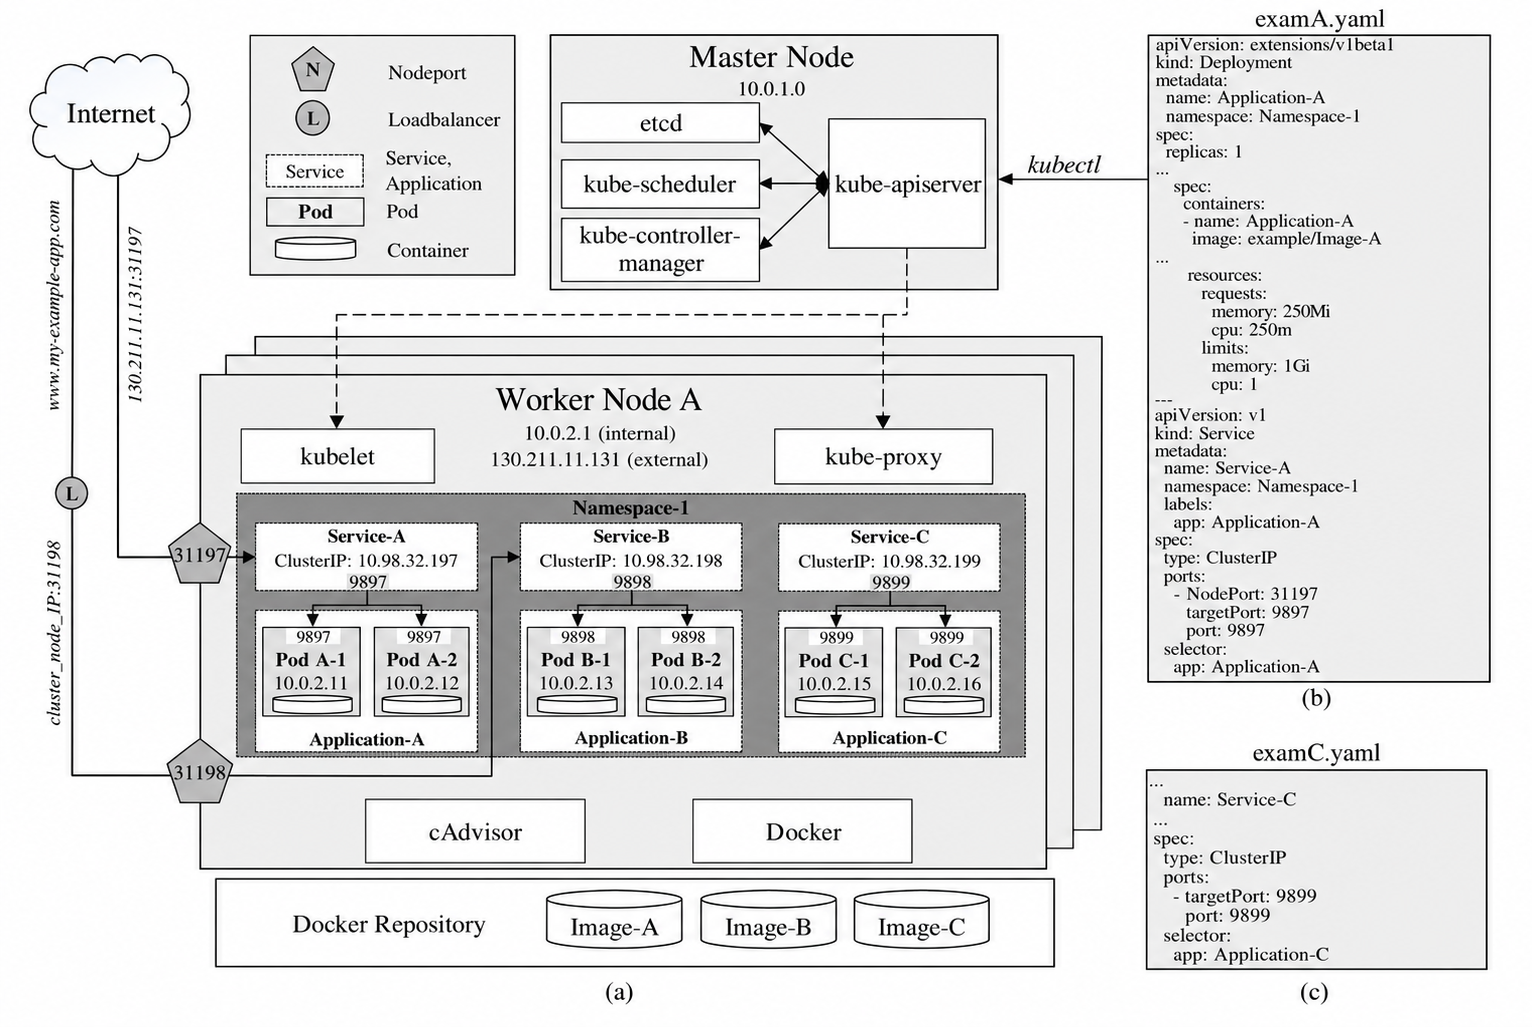
\includegraphics[width=0.85\textwidth]{figures/K8-hpa-architecuture.png}
\caption{Standard Kubernetes HPA feedback loop architecture, reproduced from Nguyen et
al.~\cite{nguyen2020hpa}. The HPA controller periodically reads aggregated resource
metrics from the API server (sourced either from the Metrics Server for KRM or the
Prometheus Adapter for PCM) and computes a desired replica count using
Equation~\ref{eq:hpa}. This loop assumes the observed metric faithfully represents
current workload intensity - an assumption that breaks down for persistent-connection
workloads where connections persist independently of CPU utilization.}
\label{fig:hpa_arch}
\end{figure*}

Figure~\ref{fig:hpa_arch} illustrates the HPA feedback loop. The controller implements
the following discrete-time proportional control law evaluated every 15~seconds (the
default synchronization period):
\begin{equation}
\textit{desiredReplicas} = \left\lceil \textit{currentReplicas} \times
  \frac{\textit{currentMetricValue}}{\textit{targetMetricValue}} \right\rceil
\label{eq:hpa}
\end{equation}

This formulation implicitly assumes that \texttt{currentMetricValue} faithfully reflects
workload intensity across all running replicas. For CPU-based scaling of stateless
workloads, this assumption generally holds. For persistent-connection workloads, it
breaks down: idle connections consume negligible CPU yet represent committed session
state whose disruption is visible to end clients. The experimental question is
therefore: \textbf{what are the consequences of this control design when the assumed
signal-to-demand coupling is absent?}



%% ============================================================
\section{Empirical Evidence of HPA Failure for Stateful WebSocket Workloads}
\label{sec:problem}
%% ============================================================

We present a controlled, progressive chain of experiments designed to isolate and characterize
each failure mode of CPU-based HPA when applied to persistent WebSocket workloads. The
experiments are ordered from least severe (over-provisioning) to most severe (permanent
connection destruction), with each experiment building upon the instrumentation and findings
of its predecessor.

All WebSocket experiments share a common infrastructure: a 3-node Kind cluster (1
control-plane + 2 worker nodes, Kubernetes v1.31.6, kind v0.25.0, configured via
\texttt{kind.yml})~\cite{kind_docs}. The Metrics Server is patched with
\texttt{--metric-resolution=15s} and \texttt{--kubelet-insecure-tls} (required for kind's
self-signed kubelet certificates; not appropriate for production). All experimental scripts,
cluster configuration, server code, load generator, and raw results are available at:
\url{https://github.com/MistaHolmes/ws-k8-controller.git}. The shared experimental infrastructure
comprises: a custom Python asyncio WebSocket server (image: \texttt{ws-instrumented}), 800
persistent client connections established by the load generator, and Kubernetes HPA configured
with \texttt{targetCPUUtilizationPercentage: 60} unless stated otherwise.

\paragraph{Instrumented server: definition and rationale}
By ``instrumented'' we mean the server was extended to expose Prometheus-format metrics
(notably a gauge \texttt{active\_connections} and a counter \texttt{new\_connections\_total})
and a minimal control endpoint (for example, \texttt{/drain}) to enable graceful handoff.
This instrumentation was adopted to obtain direct, low-latency visibility into live session
counts and connection churn - signals that CPU does not capture. The approach (i)~supplies
a precise measurement signal for storm rate computation, (ii)~permits reproducible measurement
of reconnection storms via PromQL \texttt{rate()} on \texttt{new\_connections\_total}, and
(iii)~is minimally invasive and portable.

\subsection{Experiment A: HPA Baseline Under Monotonic Correlated Load}

\paragraph{Hypothesis.} Under steady, monotonically increasing WebSocket load in which each
connection actively generates CPU work (\texttt{CPU\_WORK=1}), HPA will correctly scale the
deployment, establishing an empirical baseline for comparison with subsequent experiments.

\paragraph{Experimental Setup.} Eight hundred WebSocket clients connect incrementally over
300~seconds. Each server-side message receipt triggers a bounded CPU spin loop, maintaining
strict proportionality between active connection count and CPU utilization: CPU $\propto$
connections. HPA was configured with \texttt{minReplicas=2}, \texttt{maxReplicas=10}, and
\texttt{targetCPUUtilizationPercentage=60}.

\paragraph{Results.} As shown in Figure~\ref{fig:exp_a_replicas}, HPA scaled the deployment
monotonically from 2 to 5 replicas as CPU rose proportionally with connection count. Following
complete load removal, the system enforced the default 300-second scale-down stabilization
window before descending cleanly to \texttt{minReplicas}. No oscillatory behavior or
reconnection disruption was observed.

\begin{figure}[ht]
\centering
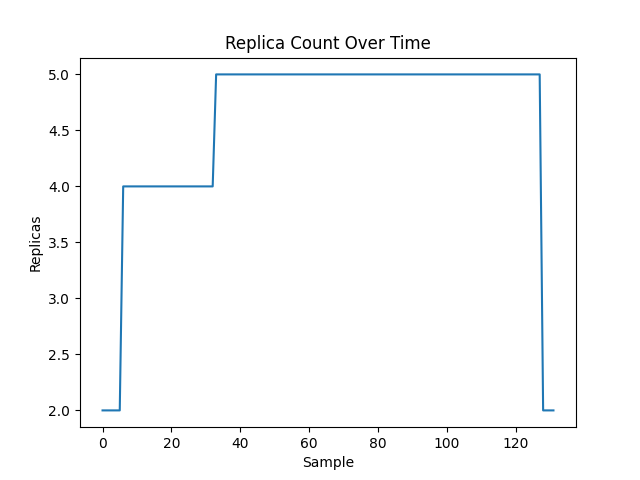
\includegraphics[width=\columnwidth]{figures/experiment-a-hpa/replicas.png}
\caption{Experiment A: Replica count timeline under monotonic WebSocket load with CPU
$\propto$ connections. The clean staircase ascent (2$\rightarrow$5), flat stabilization
plateau, and controlled descent to the minimum represent the theoretical ideal for HPA -
achievable only under perfect signal-to-demand correlation.}
\label{fig:exp_a_replicas}
\end{figure}

The replica timeline (Figure~\ref{fig:exp_a_replicas}) confirms that HPA operates correctly
\textit{when its signal accurately encodes workload demand}. Crucially, this experiment
represents a best-case scenario that is rarely achievable in production WebSocket
deployments, where connection activity levels are typically decoupled from CPU consumption.

\begin{keyresult}
\noindent\textbf{Conclusion.} CPU-based HPA functions correctly only under the idealized
condition of perfect CPU-to-connection proportionality. Subsequent experiments systematically
invalidate this condition.
\end{keyresult}

\subsection{Experiment B1: HPA Under Cyclic Load - Over-Provisioning and Recovery
Asymmetry}

\paragraph{Hypothesis.} Under realistic cyclic HIGH/LOW load patterns that simulate natural
connection activity fluctuations, HPA will exhibit systematic over-provisioning and
asymmetrically slow resource recovery.

\paragraph{Experimental Setup.} Load alternates between HIGH phases (800 connections, active
CPU-generating pinging, 60-second duration) and LOW phases (connections held persistently
idle, no pinging activity, 30-second duration). Crucially, during LOW phases the 800 client
connections remain open; only the periodic ping messages cease, collapsing CPU utilization
toward zero while connection state is preserved. Parameters were adjusted to
\texttt{maxReplicas=15} to allow unconstrained scale-up. The HPA stabilization window was
kept at the Kubernetes default of 300~seconds for scale-down
(\texttt{stabilizationWindowSeconds: 300}), intentionally unmodified to evaluate HPA behavior
under factory settings for cyclic load. Five consecutive HIGH/LOW cycles (60~s HIGH + 30~s LOW
= 90-second period) were run, for a total active cycle phase of 450~seconds.

\paragraph{Results.} During HIGH phases, HPA exhausted \texttt{maxReplicas=15} within
99~seconds - a factor of $1.875\times$ the theoretically correct value of 8~replicas
($\lceil800/100\rceil$). The core mechanism driving over-provisioning is the interaction
between the 90-second cycle period and the 300-second stabilization window: each LOW phase
(30~s) ends before the window has elapsed, so every new HIGH phase begins with the replica
count still at or near the ceiling from the previous cycle. Over five cycles, the replica
count ratchets to \texttt{maxReplicas} and remains there, with each brief LOW phase failing
to provide enough sustained low-CPU time for HPA to authorize a descent. Convergence to
\texttt{minReplicas} following the final cycle required approximately 650~seconds. The replica
count timeline (Figure~\ref{fig:exp_b1_replicas}) exhibits the expected ratcheting saturation
pattern.

\begin{figure}[ht]
\centering

\includegraphics[width=\columnwidth]{figures/experiment-b1-hpa-churn/replicas.png}
\caption{Experiment B1: HPA saturates at \texttt{maxReplicas=15} within 99~seconds under
cyclic load, representing an 87.5\% over-provision relative to the connection-derived
optimum of 8~replicas. Recovery to the minimum requires $\sim$650~seconds, demonstrating
severe asymmetry between scale-up and scale-down responsiveness.}
\label{fig:exp_b1_replicas}
\end{figure}

\begin{keyresult}
\noindent\textbf{Conclusion.} Cyclic workloads expose HPA's inability to distinguish
connection-holding periods (where CPU is low but capacity is required) from genuinely idle
periods (where capacity can be safely released). The 87.5\% over-provisioning rate and
disproportionate recovery time ($\sim$650~s) represent significant resource efficiency
penalties in production deployments.
\end{keyresult}

\subsection{Experiment B2-Instrumented: Quantifying Reconnection Storm Intensity}

\paragraph{Methodological note: supersession of a non-instrumented pilot}
Prior to this experiment, a preliminary non-instrumented variant (B2-Extended LOW) was
conducted in which the LOW phase was extended beyond the default 300-second stabilization
window to force HPA to \texttt{minReplicas=2}. While this pilot confirmed that active
connections were being severed during scale-down events through qualitative observation of
client disconnects, it produced no quantitative data: the server exposed no Prometheus
metrics, connection loss counts were unverifiable, and reconnection rates were entirely
unobservable. The pilot served its intended engineering purpose - confirming the failure
mode was reproducible before investing in full instrumentation - but it contributes no
independent publishable evidence beyond what B2-Instrumented already provides with greater
precision. Accordingly, B2-Extended LOW is not reported as a standalone experiment in this
paper. Its sole scientific contribution is as the direct motivation for adding the Prometheus
instrumentation described below.

\paragraph{Hypothesis.} Each HPA scale-down event, by terminating pods hosting active
connections, will trigger a measurable reconnection storm with peak rates exceeding
1,000~connections/second, and will induce overshoot of the steady-state connection target
due to the cascade of concurrent reconnection attempts.

\paragraph{Experimental Setup.} The WebSocket server was instrumented with two Prometheus
metrics: \texttt{active\_connections} (a gauge reflecting current session count) and
\texttt{new\_connections\_total} (a monotonically increasing counter enabling rate computation
via \texttt{rate()}). Prometheus was configured to scrape at a 15-second interval. The HPA
policy was configured with \texttt{stabilizationWindowSeconds: 0} for scale-up and
\texttt{stabilizationWindowSeconds: 60} for scale-down. Setting scale-up to zero ensures that
each reconnection storm (which spikes CPU) immediately triggers scale-up, guaranteeing that
every cycle produces a complete and observable scale-up/scale-down sequence within the
measurement window. Each cycle consisted of a 60-second HIGH phase (800 pinging clients,
\texttt{CPU\_WORK=1}) followed by a 90-second LOW phase (connections idle, no pinging). The
90-second LOW duration was specifically chosen to exceed the 60-second scale-down stabilization
window, ensuring that HPA always executes at least one scale-down event per cycle. Five
complete HIGH/LOW cycles were executed.

\paragraph{Results.} Every HPA scale-down event across all five cycles triggered a distinct,
measurable reconnection storm. Storm rates were highly consistent: Cycle~1:
1,400.9~conn/s; Cycle~2: 1,298.3~conn/s; Cycle~3: 1,399.5~conn/s; Cycle~4: 1,251.8~conn/s;
Cycle~5 trailed as the connection population had partially degraded. The peak reconnection
rate reached \textbf{1,400~connections/second}, as shown in
Figure~\ref{fig:exp_b2_reconnections}. Concurrent with each storm, the active connection
count transiently overshot the 800-connection steady-state target, peaking at \textbf{1,215
connections} - a 51.9\% overshoot (Figure~\ref{fig:exp_b2_connections}).

The socket-level mechanism driving this overshoot is as follows: when a pod is sent
\texttt{SIGKILL} after its 30-second termination grace period, its TCP connections are
abruptly reset (TCP RST). All 800 clients detect closure simultaneously and immediately
initiate reconnection. The Prometheus gauge \texttt{active\_connections} on the surviving
pods begins counting new incoming connections before the OS completes cleanup of socket state
(including the TIME\_WAIT window for recently reset connections), transiently reporting a
total above the 800-client ceiling. The overshoot resolves within 15--30~seconds as OS-level
socket reclaim completes.

\begin{figure}[ht]
\centering
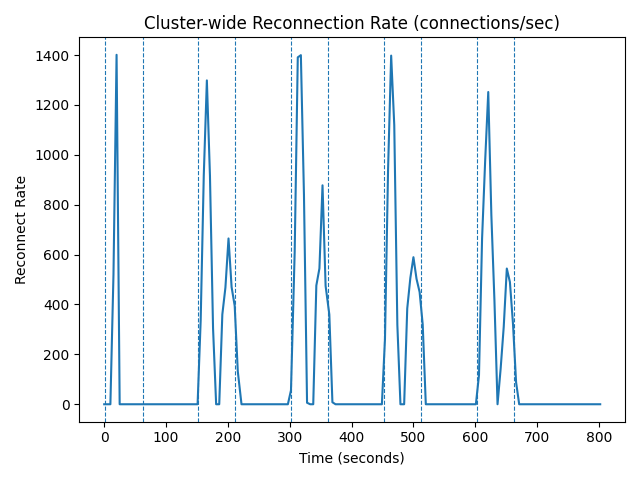
\includegraphics[width=\columnwidth]{figures/experiment-b2-hpa-churn-instrumented/reconnections.png}
\caption{Experiment B2-Instrumented: Prometheus-measured reconnection rate
(\texttt{rate(new\_connections\_total[15s])}) over the five-cycle experiment. Each
reconnection spike is precisely synchronized with an HPA scale-down event, with peak
observed rates of 1,400~connections/second.}
\label{fig:exp_b2_reconnections}
\end{figure}

\begin{figure}[ht]
\centering

\includegraphics[width=\columnwidth]{figures/experiment-b2-hpa-churn-instrumented/connections.png}
\caption{Experiment B2-Instrumented: Active connection count during the reconnection storm
period. The connection overshoot of 1,215 (51.9\% above the 800-client target) arises as
reconnecting clients establish new sessions before the server has fully released the state
associated with severed connections.}
\label{fig:exp_b2_connections}
\end{figure}

Figure~\ref{fig:exp_b2_scaling} provides the combined view of replica oscillation and
connection disruption, establishing the causal chain from HPA scaling decision to client-side
session disruption.

\begin{figure}[ht]
\centering
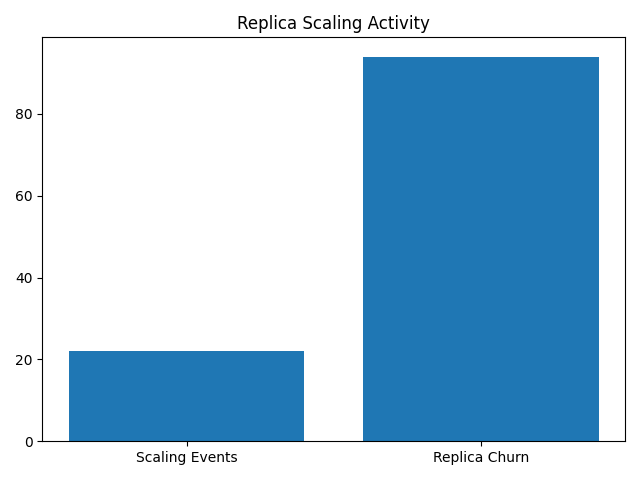
\includegraphics[width=\columnwidth]{figures/experiment-b2-hpa-churn-instrumented/scaling_activity.png}
\caption{Experiment B2-Instrumented: Temporal correlation between HPA replica changes
(green) and active connection count (blue). Each downward step in replicas corresponds to
a measurable spike in the connection disruption signal, confirming the direct causal
relationship.}
\label{fig:exp_b2_scaling}
\end{figure}

\begin{keyresult}
\noindent\textbf{Conclusion.} In our experiments, every HPA scale-down event was destructive
to WebSocket client sessions. Each replica reduction severed all connections hosted on the
terminated pod, producing a reconnection storm whose intensity scaled with the connection
density of the removed replica. At 1,400~conn/s, such storms represent a significant
degradation event for latency-sensitive applications.
\end{keyresult}

\subsection{Experiment B3: Permanent Connection Loss Under Non-Reconnecting Clients}
\label{sec:b3}

\paragraph{Hypothesis.} When WebSocket clients do not implement reconnection logic -
modeling clients that treat connection loss as a terminal failure (e.g., batch data
collectors, embedded IoT sensors, or long-running streaming sessions) - HPA scale-down
events will cause \textit{permanent, irrecoverable reduction} in the total session population.

\paragraph{Experimental Setup.} The load generator was reconfigured with
\texttt{reconnect: false}. Once a client's connection is severed by pod termination, the
client neither retries nor reconnects. The HPA policy mirrored B2-Instrumented:
\texttt{stabilizationWindowSeconds: 0} for scale-up and \texttt{stabilizationWindowSeconds:
60} for scale-down. CPU work was retained (\texttt{CPU\_WORK=1}) to maintain HPA activity.
The IDLE phase runs for up to 240~seconds (\texttt{IDLE\_MAX\_DURATION=240}), providing
sufficient headroom for HPA to execute multiple sequential scale-down events.

\paragraph{Pod termination mechanics and the 30-second limbo}
Understanding the exact Kubernetes pod termination sequence is essential for interpreting
this experiment. When HPA reduces \texttt{spec.replicas}, the following steps occur in
order: (1)~the target pod is immediately removed from the Service's endpoint slice, so no
new connections are routed to it; (2)~Kubernetes sends \texttt{SIGTERM} to the pod's main
process and starts the \texttt{terminationGracePeriodSeconds} timer (default: 30~s);
(3)~during the 30-second grace period, existing TCP connections on the terminating pod remain
open and functional - they are maintained by the OS kernel, not Kubernetes; (4)~after
\texttt{terminationGracePeriodSeconds} elapses, Kubernetes sends \texttt{SIGKILL}, which
tears down the process and the OS forcibly resets all open TCP connections (TCP RST). This
sequence is why the active connection drop visible in Figure~\ref{fig:exp_b3_connections}
lags behind HPA's scale-down decision by approximately 30~seconds: the connection is not
immediately destroyed when HPA acts, but is destroyed 30~seconds later when
\texttt{SIGKILL} fires. This delay does not mitigate the harm - the connection still dies,
the client still receives a TCP RST, and with \texttt{reconnect: false}, the session is
permanently lost.

\paragraph{Results.} The active connection count (Figure~\ref{fig:exp_b3_connections})
exhibits a characteristic \textbf{staircase step-down} pattern. Each step corresponds
precisely to an HPA scale-down decision: when a pod is terminated, the full contents of its
connection table are permanently destroyed. Successive scale-down events cause monotonically
fewer active connections, with no mechanism for recovery. The representative run (Run~4
of the five-run replication; see Table~\ref{tab:b3_replication}) exhibits the trajectory
$800 \rightarrow 771 \rightarrow 708 \rightarrow 644$, a 19.5\% permanent loss.

\begin{figure*}[t]
\centering

\includegraphics[width=0.85\textwidth]{figures/experiment-b3-hpa-idle-connections/connections.png}
\caption{Experiment B3 (representative Run~4): Active connection count exhibits permanent
staircase destruction ($800{\rightarrow}771{\rightarrow}708{\rightarrow}644$). Each
step-down is precisely synchronized with an HPA scale-down event. The connections are
irrecoverable under the \texttt{reconnect: false} regimen. Across all five replications,
the mean final connection count was $649.4 \pm 8.8$ (Table~\ref{tab:b3_replication}).}
\label{fig:exp_b3_connections}
\end{figure*}

The combined view in Figure~\ref{fig:exp_b3_combined} illustrates the causal chain:
(1)~connections become idle and cease to generate CPU load; (2)~HPA, observing near-zero CPU,
decides to scale down; (3)~the terminated pod destroys all connections it hosts permanently.
This behavior is not addressable through configuration parameter changes - it arises from
HPA's inability to observe connection state as a first-class scaling signal.

\begin{figure*}[t]
\centering

\includegraphics[width=0.85\textwidth]{figures/experiment-b3-hpa-idle-connections/combined.png}
\caption{Experiment B3, combined signal view - the causal proof of the mismatch between
CPU-based scaling signals and stateful workload characteristics. CPU utilization (red) drops
to near zero as connections become idle $\rightarrow$ HPA scales down the replica count
(green) $\rightarrow$ active connections (blue) are permanently destroyed. The autoscaler is
induced by its own metric to destroy the session state it should be protecting.}
\label{fig:exp_b3_combined}
\end{figure*}

\begin{keyresult}
\noindent\textbf{Conclusion.} The reliance of HPA on CPU as a scaling signal causes
the autoscaler to act against the interests of idle-but-connected stateful workloads. Our
findings suggest that the problem is unlikely to be remediated by parameter tuning alone
and motivates the exploration of alternative scaling architectures.
\end{keyresult}

\paragraph{Replication and Statistical Validation}
To ensure the observed staircase destruction is robust and not a transient artifact,
Experiment~B3 was replicated five times under identical conditions: the same Kind cluster
configuration, the same HPA policy (\texttt{stabilizationWindowSeconds: 60} for
scale-down), 800 non-reconnecting clients, and the same two-phase protocol
(120-second CONNECT phase followed by a 240-second IDLE phase). Each run used a
freshly provisioned cluster to eliminate state carry-over between replications.
Table~\ref{tab:b3_replication} summarizes the per-run connection counts and loss
percentages, while Table~\ref{tab:b3_steps} provides the active connection count
at each observed staircase step for every run.

\begin{table}[ht]
\centering
\caption{Statistical replication of Experiment B3 (5 runs). Peak connections reached
800 in all runs, while final connection counts exhibited consistent degradation due to
scale-down events, averaging 18.8\% connection loss per run.}
\label{tab:b3_replication}
\begin{tabular}{@{}lccc@{}}
\toprule
\textbf{Run} & \textbf{Peak Conn.} & \textbf{Final Conn.} & \textbf{Loss (\%)} \\
\midrule
Run 1 & 800 & 637 & 20.4\% \\
Run 2 & 800 & 652 & 18.5\% \\
Run 3 & 800 & 658 & 17.8\% \\
Run 4 & 800 & 644 & 19.5\% \\
Run 5 & 800 & 656 & 18.0\% \\
\midrule
\textbf{Mean $\pm$ SD} & \textbf{800 $\pm$ 0} & \textbf{649.4 $\pm$ 8.8} & \textbf{18.8\% $\pm$ 1.1\%} \\
\bottomrule
\end{tabular}
\end{table}

\begin{table}[ht]
\centering
\caption{Active connection count at each observed staircase step during the IDLE phase
for all five B3 replications. Each step-down corresponds to a distinct HPA scale-down
event that permanently destroyed the connections hosted on the terminated pod.}
\label{tab:b3_steps}
\begin{tabular}{@{}lcccc@{}}
\toprule
\textbf{Run} & \textbf{Step 0} & \textbf{Step 1} & \textbf{Step 2} & \textbf{Final} \\
\midrule
Run 1 & 800 & 740 & -- & 637 \\
Run 2 & 800 & 718 & 686 & 652 \\
Run 3 & 800 & 761 & 668 & 658 \\
Run 4 & 800 & 771 & 708 & 644 \\
Run 5 & 800 & 741 & 735 & 656 \\
\bottomrule
\end{tabular}
\end{table}

Several observations strengthen the claim that the staircase destruction pattern is a
deterministic consequence of HPA's architecture rather than a stochastic artifact:

\begin{enumerate}[leftmargin=*]
\item \textbf{Consistency of the destruction magnitude.} The final connection count
across all five runs falls within a narrow band of 637--658, yielding a standard
deviation of only 8.8~connections (1.1\% in loss percentage). This low variance
confirms that the number of connections destroyed per scale-down event is governed
by the deterministic connection distribution across pods rather than by random
fluctuation.

\item \textbf{Qualitative uniformity of the staircase pattern.} Every run exhibits
the same three-phase trajectory: (i)~monotonic ramp from 0 to 800 during the CONNECT
phase, (ii)~a brief plateau at 800 while CPU is still elevated, and (iii)~a staircase
descent once CPU drops and HPA begins scaling down. The number of intermediate steps
varies between 2 and 3 depending on the timing of HPA's evaluation cycle relative to
the IDLE phase onset, but the qualitative pattern is invariant.

\item \textbf{Per-step connection loss.} Each individual scale-down step destroys
between 6 and 163~connections, corresponding to the full connection table of the
terminated pod. The variation in per-step loss reflects the uneven distribution of
connections across pods imposed by Kubernetes' round-robin Service routing, not any
non-determinism in the HPA control loop.
\end{enumerate}

\subsection{Summary of the Evidence Chain}

Table~\ref{tab:failure_summary} consolidates the progressive evidence across all four HPA
experiments.

\begin{table*}[t]
\centering
\caption{Summary of the progressive evidence chain demonstrating the failure of CPU-based
HPA for stateful WebSocket workloads. Each experiment isolates and quantifies a distinct
failure mode.}
\label{tab:failure_summary}
\begin{tabular}{@{}p{2.2cm}p{3.5cm}p{3.5cm}p{5cm}@{}}
\toprule
\rowcolor{gray!12}
\textbf{Experiment} & \textbf{Condition} & \textbf{HPA Behavior} & \textbf{Key Quantitative Finding} \\
\midrule
A (Baseline) & Monotonic load; CPU $\propto$ connections & Correct proportional scaling & Works only under idealized signal correlation \\
B1 (Cyclic) & Alternating HIGH/LOW activity & Reaches \texttt{maxReplicas} in 99~s & 87.5\% over-provisioning; 650~s to recover \\
B2-Inst. (Measured) & Cyclic + Prometheus instrumentation & Reconnection storm per scale-down & Peak 1,400~conn/s; 51.9\% connection overshoot \\
B3 (No-reconnect) & Idle connections; no client retry & Permanent, staircase connection loss & $800{\rightarrow}649$ mean final (18.8\% loss); zero recovery \\
\bottomrule
\end{tabular}
\end{table*}



%% ============================================================
\section{Discussion}
\label{sec:discussion}
%% ============================================================

\subsection{CPU as an Invalid Scaling Signal for Stateful Workloads}
\label{sec:signal_mismatch}

The fundamental architectural mismatch can be stated precisely using two formal
definitions. Let $M(t)$ denote the \textit{scaling metric} observed by HPA at time
$t$ -- in the standard configuration, $M(t)$ is the average CPU utilization across
all running replicas. Let $D(t)$ denote the \textit{true workload demand} at time
$t$, defined as the number of active connections $C(t)$ that require server-side
session state to be preserved. The HPA proportional control law
(Equation~\ref{eq:hpa}) computes the desired replica count from $M(t)$, implicitly
assuming that the scaling metric is a faithful proxy for workload demand:
\begin{equation}
M(t) \propto D(t) \quad \Longrightarrow \quad
\textit{desiredReplicas}(t) \propto D(t)
\label{eq:hpa_assumption}
\end{equation}
Under this assumption, scaling decisions derived from $M(t)$ correctly track the
true capacity requirement. For stateless HTTP workloads where each request consumes
a bounded CPU quantum and releases it upon completion, the proportionality
$M(t) \propto D(t)$ holds empirically (as confirmed by Experiment~A).

For persistent-connection workloads with idle phases, however, this assumption is
violated in a specific and destructive manner. During active phases, connections
generate CPU work and the proportionality holds; during idle phases, the connections
persist (demand $D(t) = C(t) > 0$) but cease generating CPU load, causing the
observed metric to collapse:
\begin{equation}
M(t) \to 0 \quad \text{while} \quad D(t) = C(t) > 0
\label{eq:websocket_reality}
\end{equation}
The consequence is immediate: HPA computes
$\textit{desiredReplicas} \approx \textit{minReplicas}$ (via Equation~\ref{eq:hpa})
and initiates scale-down, destroying the connections hosted on the terminated pods.
Equation~\ref{eq:websocket_reality} is not a marginal degradation of the
proportionality in Equation~\ref{eq:hpa_assumption} -- it is a complete decoupling
of the signal from the demand, producing a scaling decision that is maximally wrong
(scale down to minimum while demand is at maximum).

The evidence chain from Experiments~B1, B2-Instrumented, and B3 collectively indicates
that CPU utilization is a poor proxy for WebSocket workload intensity, and in the cases
we tested, an actively misleading one.
In Experiment~B3, CPU dropped to near-zero precisely because connections were idle, triggering
HPA to terminate the pods hosting those connections. This creates a circular
destruction pattern: the metric signal drops $\rightarrow$ HPA scales down $\rightarrow$
session state is destroyed. The autoscaler is induced by its own metric to destroy the very
resource it should be protecting.

The companion paper demonstrates this converse: a controller operating at \texttt{CPU\_WORK=0}
throughout 570~seconds correctly maintains 8~replicas based solely on the connection count
signal. This result confirms that the failure resides in the signal, not in the control
algorithm: a perfect proportional controller on the wrong signal produces worse outcomes than
a simpler controller on the correct signal.

\subsection{The Stabilization Window Semantic Mismatch}

A natural response to the evidence presented here is to ask whether tuning HPA's built-in
stabilization window to a sufficiently large value would protect idle connections. Our
analysis indicates this is unlikely to succeed, for a semantic reason.

HPA's stabilization window buffers a time series of \textit{desiredReplicas} values computed
from CPU observations. When connections are idle and CPU reads near-zero persistently, every
entry in HPA's window recommends \texttt{minReplicas}. The stabilized output - the maximum
over all window entries - therefore converges to \texttt{minReplicas} regardless of how long
the window is extended. A longer window merely delays the convergence; it does not retain
the information that connections
were present.

The correct stabilization mechanism must buffer \textit{connection-derived desired counts}:
it must retain the high-water mark of recently required capacity, computed from the connection
metric rather than from CPU. This is a semantic difference, not a parameter difference. The
companion paper implements and evaluates such a mechanism experimentally.

\subsection{The 30-Second Limbo Window as a Design Constraint}

The Kubernetes pod termination sequence creates a 30-second limbo window between
\texttt{SIGTERM} and \texttt{SIGKILL} during which connections survive at the OS level but
are doomed. This window is commonly proposed as an opportunity for graceful drain via
\texttt{preStop} hooks. For WebSocket workloads with session durations of minutes to hours,
30~seconds is typically insufficient for connection migration or drain.

The correct mitigation is not a longer termination period but rather \textit{scale-down
suppression} - preventing the scale-down decision from being made in the first place while
live sessions are present. Any viable autoscaling solution for persistent-connection workloads
must incorporate this principle.

\subsection{HPA Stabilization Window Tuning Study}
\label{sec:tuning_study}

A natural hypothesis is that HPA's destructive behavior during idle phases could be
mitigated by aggressively tuning the \texttt{scaleDown.stabilizationWindowSeconds}
parameter to outlast the expected idle gap. To evaluate this claim empirically, we
conducted a systematic tuning study spanning four stabilization window sizes --
30, 60, 120, and 300~seconds -- each tested under two gap conditions.

\paragraph{Experimental Methodology.}
For each window value $W \in \{30, 60, 120, 300\}$~seconds, we ran the B3 workload
protocol (800 non-reconnecting clients, 120-second CONNECT phase with
\texttt{CPU\_WORK=1}) followed by an idle gap of duration $G$. Two gap conditions
were tested per window: (i)~$G < W$ (``below''), where the idle gap is shorter than
the stabilization window and connections should be protected; and (ii)~$G > W$
(``above''), where the idle gap exceeds the window and HPA is expected to execute a
scale-down. The specific gap durations were chosen as $G_{\text{below}} = W - 15$~s
and $G_{\text{above}} = W \times 1.5$ to $W + 60$~s, providing margin on both sides
of the window boundary. Each of the eight configurations (4 windows $\times$ 2 gap
conditions) was replicated three times on freshly provisioned Kind clusters, yielding
24~sub-experiments in total.

\paragraph{Results.}
Table~\ref{tab:tuning_results} presents the aggregated results across all
configurations. The pattern is unambiguous: when the idle gap falls below the
stabilization window, connections are universally preserved (0\% loss across all
12~below-window runs). When the gap exceeds the window, connection destruction
occurs in every configuration, with mean loss rates ranging from 5.2\% (30-second
window) to 33.2\% (300-second window).

\begin{table}[ht]
\centering
\caption{HPA stabilization window tuning study results (3 replications per
configuration). Gap relation indicates whether the idle gap duration was below
or above the configured stabilization window. Connection loss is reported as
mean $\pm$ SD across the three runs.}
\label{tab:tuning_results}
\begin{tabular}{@{}cccrr@{}}
\toprule
\textbf{Window} & \textbf{Gap} & \textbf{Relation} & \textbf{Loss (\%)} & \textbf{Survived} \\
\midrule
30s  & 15s  & below & $0.0 \pm 0.0$ & 3/3 \\
30s  & 90s  & above & $5.2 \pm 6.2$ & 2/3 \\
\midrule
60s  & 45s  & below & $0.0 \pm 0.0$ & 3/3 \\
60s  & 120s & above & $10.2 \pm 7.2$ & 2/3 \\
\midrule
120s & 105s & below & $0.0 \pm 0.3$ & 3/3 \\
120s & 180s & above & $10.4 \pm 5.6$ & 1/3 \\
\midrule
300s & 285s & below & $0.0 \pm 0.0$ & 3/3 \\
300s & 360s & above & $33.2 \pm 28.0$ & 1/3 \\
\bottomrule
\end{tabular}
\end{table}

\begin{figure}[ht]
\centering
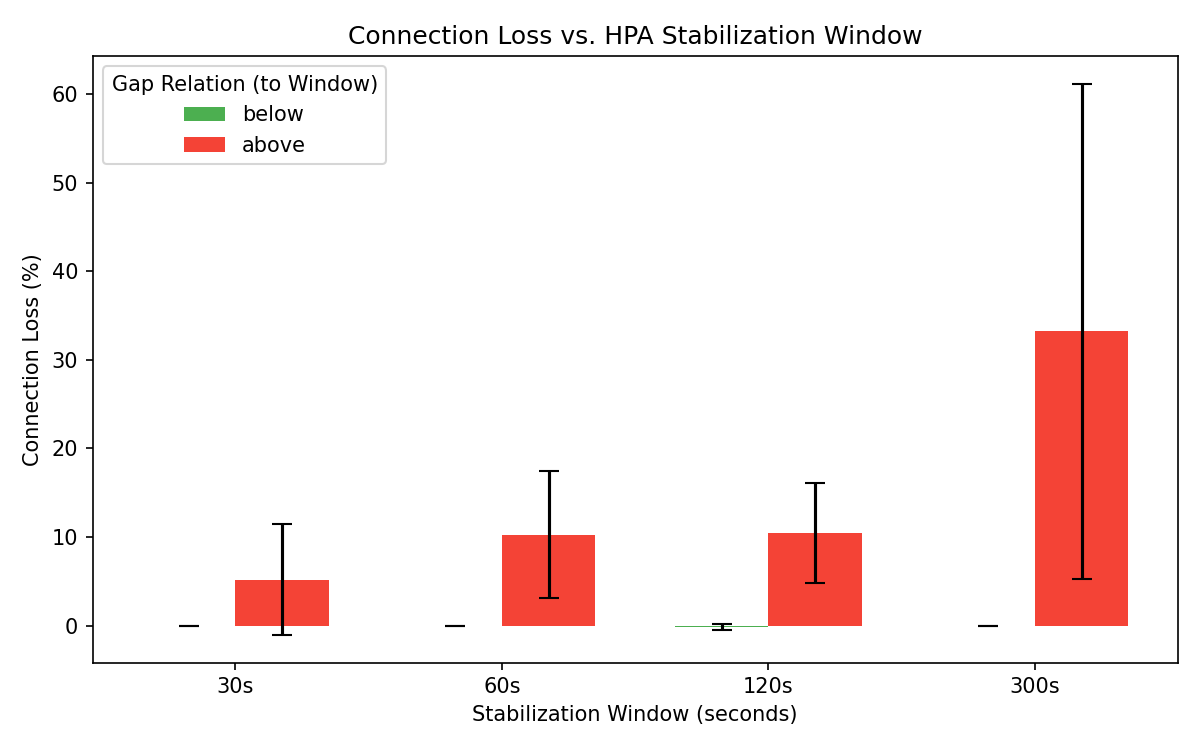
\includegraphics[width=\columnwidth]{figures/tuning_results_loss.png}
\caption{Connection loss percentage relative to the HPA stabilization window and
gap duration. Green bars (``below'') show zero loss when the gap is shorter than
the window; red bars (``above'') show consistent connection destruction when the
gap exceeds the window, regardless of window size.}
\label{fig:tuning_results}
\end{figure}

\paragraph{Analysis.}
The results confirm two critical properties of HPA's stabilization mechanism.
First, the stabilization window functions as a \textit{delay}, not a
\textit{protection} mechanism: it defers the scale-down decision for $W$~seconds
but does not prevent it. As long as CPU remains near zero throughout the window
period, every entry in the window's recommendation buffer converges to
\texttt{minReplicas}, and the stabilized output (the maximum over the window)
eventually equals \texttt{minReplicas}.

Second, the increasing variance in the ``above'' condition at larger window values
(SD = 28.0\% at $W=300$s vs.\ SD = 6.2\% at $W=30$s) reflects the non-deterministic
timing of HPA's 15-second evaluation cycle relative to the window boundary. When the
gap only marginally exceeds the window, whether scale-down occurs within the
measurement period depends on the alignment of the HPA sync cycle with the gap
transition -- a source of measurement variance, not of protection.

The tuning study conclusively establishes that the stabilization window is
insufficient to protect idle connections: it is a temporal buffer on
CPU-derived recommendations, not a connection-aware protection mechanism.
No finite window value can prevent scale-down when the underlying metric
persistently reads zero.

%% ============================================================
\section{Limitations}
\label{sec:limitations}
%% ============================================================

\begin{enumerate}[leftmargin=*]

\item \textbf{Evaluation environment.} All experiments were conducted on a single-machine
Kind cluster. While this provides full reproducibility and controlled conditions, it does not
capture cross-node scheduling latency, network partitions, or metric-collection noise present
in multi-node cloud clusters. Results are directionally valid; absolute timing values
(e.g., pod startup lag, HPA sync precision) may differ on production infrastructure.

\item \textbf{Workload generalizability.} The load generator uses synthetic WebSocket
workloads with a linear connection ramp and deterministic silence gaps. Real-world connection
arrival is more bursty and session durations vary widely. For stationary random load (Poisson
arrivals), the proportional failure mechanisms apply unchanged; only the observed peak
connection count and storm rate would vary.

\item \textbf{Instrumentation dependency.} B2-Instrumented results depend on Prometheus
metric freshness at a 15-second scrape interval. A higher scrape interval would affect storm
rate measurement precision but would not change the causal finding that scale-down events
trigger reconnection cascades.

\item \textbf{Single reconnect=false regime.} Experiment~B3 uses a uniform
\texttt{reconnect: false} policy. Real deployments have a mix of reconnecting and
non-reconnecting clients; the staircase destruction rate and final session population would
differ under a mixed client policy.

\end{enumerate}



%% ============================================================
\section{Conclusion}
\label{sec:conclusion}
%% ============================================================

This paper presented a systematic, empirically grounded characterization of Kubernetes HPA
failure modes for stateful WebSocket workloads through a progressive chain of four controlled
experiments.

Experiment~A established that CPU-based HPA functions correctly under the idealized
condition of strict CPU-to-connection proportionality, a scenario rarely achievable
in production WebSocket deployments. Experiment~B1 demonstrated that cyclic workloads
cause HPA to over-provision by \textbf{87.5\%} (15 vs.\ the correct 8 replicas), exhausting
\texttt{maxReplicas} within 99~seconds, with recovery requiring 650~seconds. Experiment
B2-Instrumented provided a causal, Prometheus-measured quantification of reconnection
storm magnitude, observing a peak rate of \textbf{1,400~connections/second} and a 51.9\%
connection count overshoot directly synchronized with HPA scale-down events. Experiment~B3
demonstrated permanent, irrecoverable staircase connection destruction under non-reconnecting
clients, with the active session population reduced from \textbf{800 to a mean of 649}
(18.8\% loss, $\pm$1.1\% across five replications) with zero recovery, as the combined
signal view established the complete causal chain: CPU drop $\rightarrow$ scale-down
decision $\rightarrow$ permanent session destruction.

Our experiments suggest that these failure modes are \textit{architectural} rather than
configurational: they arise from the limitations of CPU as a scaling signal for
persistent-connection workloads, and are unlikely to be remediated by HPA parameter tuning
alone. Specifically, the built-in stabilization window does not protect idle connections
because it buffers CPU-derived replica recommendations rather than connection-derived
desired counts - a semantic mismatch, not a parameter mismatch.

These findings carry a direct design implication: any autoscaling solution for stateful
persistent-connection workloads must simultaneously (a) replace the scaling signal with a
connection-count metric that encodes actual session state, and (b) implement scale-down
lifecycle semantics that suppress premature termination while live sessions are present. The
companion paper presents the design, implementation, and multi-baseline experimental
validation of the \texttt{StatefulAutoscaler} - a custom Kubernetes controller that
addresses all three documented failure modes through connection-density scaling and
sliding-window stabilization.



\section*{Data Availability}

The source code, experimental workloads, Kubernetes manifests,
Prometheus configurations, analysis scripts, and processed results
required to reproduce Experiments~A, B1, B2-Instrumented, and B3
are publicly available at:

\begin{center}
\url{https://github.com/MistaHolmes/ws-k8-controller.git}
\end{center}

The repository includes deployment manifests, load-generation
workloads, raw measurement data, figure-generation scripts, and
step-by-step replication instructions. All figures presented in this
paper were generated directly from the archived experimental results.

\section*{Acknowledgements}

The authors express their sincere gratitude to Dr.\ Rakesh Kumar Ranjan
for his supervision, guidance, and constructive feedback throughout this research. His insights into experimental design, measurement methodology, and research structuring played an important role in improving both the technical rigor and presentation of this work.

The authors also thank him for his continued encouragement during the
development of the experimental framework and for facilitating access to the computational resources used to conduct the experiments and collect the reported results.

Finally, the authors acknowledge the Department of Computer Science and
Engineering, C V Raman Global University, for providing an academic
environment that supported this research.


%% ============================================================
\bibliographystyle{spbasic}
\bibliography{reference}

\end{document}